\chapter{Architecture Globale du Système}
\label{ch:archi_globale}

\section{Vue d'ensemble --- architecture telle que construite}
\label{sec:archi_overview}

Contrairement au cahier des charges initial (chapitre~\ref{ch:presentation}), l'analyse du
code source du dépôt \texttt{Esi\_Bot} révèle une architecture matérielle sensiblement
différente, organisée en trois couches de traitement et une couche d'alimentation
dédiée. La figure~\ref{fig:global_archi} reproduit le schéma d'architecture officiel
fourni par l'équipe, qui sert de référence pour ce chapitre.

\begin{figure}[H]
	\centering
	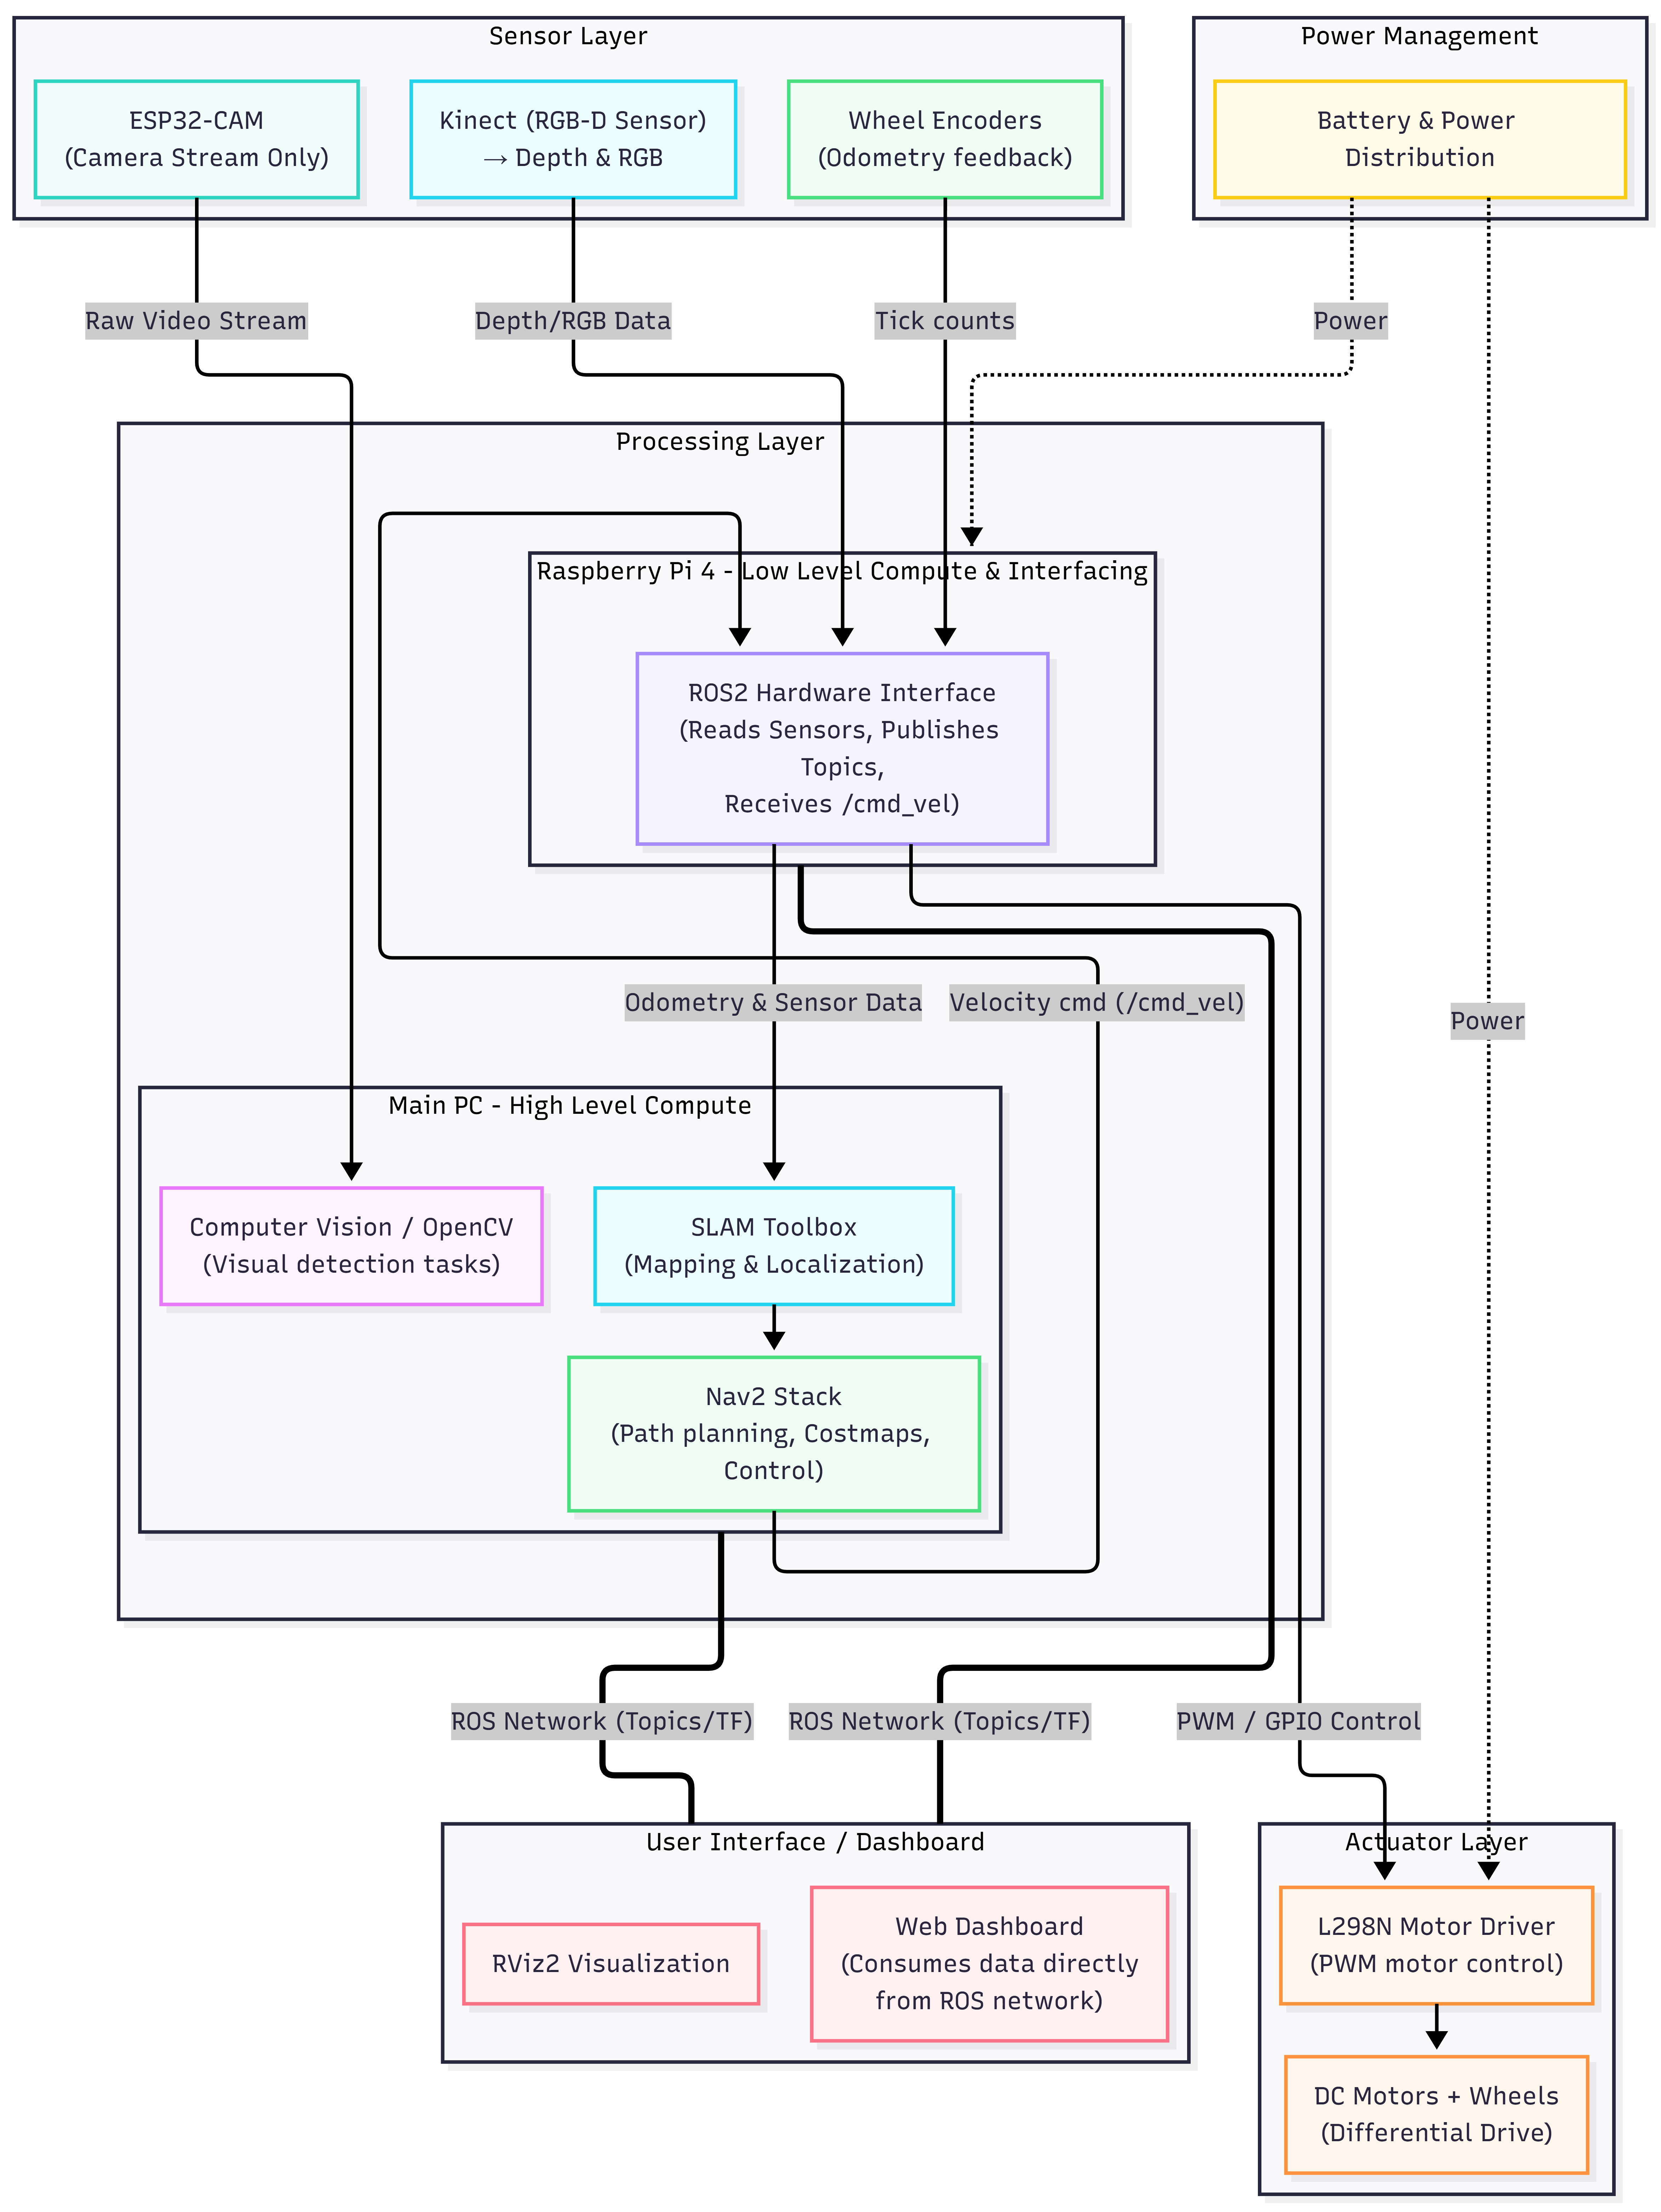
\includegraphics[width=0.62\linewidth]{images/Global_Archi.png}
	\caption{Architecture globale d'\esibot{} telle que construite (document fourni par
		l'équipe). Le capteur de cartographie principal est le Kinect (RGB-D) et non le
		radar ultrasonique du cahier des charges ; les moteurs sont pilotés directement
		par le Raspberry\,Pi\,4 et non par l'ESP32-CAM.}
	\label{fig:global_archi}
\end{figure}

Quatre observations structurantes ressortent de ce schéma et sont confirmées par le code
source~:

\begin{enumerate}
	\item \textbf{L'ESP32-CAM est réduit à une fonction unique de caméra de streaming.}
	      Le firmware \texttt{CameraServerArduinoIDE.ino} (variante du serveur de caméra
	      ESP32 standard d'Espressif, modèle \texttt{AI\_THINKER}) ne pilote ni moteurs, ni
	      servo, ni capteur de distance --- il expose uniquement un flux \gls{mjpeg} HTTP sur
	      le réseau \gls{wifi} local.
	\item \textbf{Le Raspberry\,Pi\,4 assure l'intégralité de l'interfaçage bas-niveau.} Le
	      nœud \texttt{motor\_bridge\_node} (paquet \texttt{esibot\_hardware}) pilote
	      directement le pont en H L298N et lit les encodeurs de roue via les broches
	      \gls{gpio} du Raspberry\,Pi --- une responsabilité initialement prévue pour
	      l'ESP32-CAM.
	\item \textbf{Le capteur de cartographie principal est un Kinect (v1), pas le radar
	      ultrasonique.} Le paquet \texttt{esibot\_slam} lance le pilote
	      \texttt{kinect\_ros2}, convertit son image de profondeur en balayage laser de
	      pseudo-portée via \texttt{depthimage\_to\_laserscan}, puis alimente
	      \texttt{slam\_toolbox}. Le nœud \texttt{ultrasonic\_scan\_node} existe toujours
	      dans le paquet \texttt{esibot\_sensors} mais son lancement est commenté dans le
	      script d'exploitation \texttt{start\_esibot\_all.sh} --- il s'agit donc d'un
	      chemin de code \emph{déprécié}, conservé mais non utilisé en exploitation
	      courante.
	\item \textbf{Une centrale inertielle (\gls{imu}) MPU6050} a été ajoutée, absente du
	      cahier des charges initial, et fusionnée à l'odométrie par encodeurs via un
	      filtre de Kalman étendu (\texttt{robot\_localization}), afin de stabiliser le cap
	      du robot et d'améliorer la précision de l'odométrie fournie à \gls{slam} et Nav2.
\end{enumerate}

\section{Découpage en trois couches}
\label{sec:archi_layers}

\paragraph{Couche 1 --- Capteurs (Sensor Layer).}
Trois sources de données indépendantes alimentent la couche de traitement~: l'ESP32-CAM
(flux vidéo brut \gls{mjpeg}), le Kinect (image de profondeur et image couleur RGB), et les
encodeurs de roue (comptage d'impulsions pour l'odométrie). Chaque source utilise une
interface physique distincte~: \gls{wifi} pour la caméra, USB pour le Kinect, \gls{gpio}
à interruption pour les encodeurs.

\paragraph{Couche 2 --- Traitement bas-niveau (Raspberry\,Pi\,4).}
Le Raspberry\,Pi\,4 héberge l'interface matérielle \ros{}\,2~: il lit les capteurs
embarqués (encodeurs, \gls{imu}), exécute la boucle d'asservissement de vitesse \gls{pid}
des deux moteurs, publie l'odométrie et les topics de télémétrie, et reçoit les commandes
de vitesse \topic{/cmd\_vel}.

\paragraph{Couche 3 --- Traitement haut-niveau (PC opérateur).}
Le schéma officiel positionne la vision par ordinateur (OpenCV), \pkg{slam\_toolbox} et la
pile Nav2 sur un PC principal distinct, communiquant avec le Raspberry\,Pi\,4 via le réseau
\ros{}\,2 (DDS, topics/\gls{tf}). Cette séparation logique est rendue possible par la
nature distribuée de \ros{}\,2~: les arguments de lancement
(\texttt{start\_base}, \texttt{start\_kinect}, \texttt{start\_slam}, \texttt{start\_rviz})
du fichier \texttt{mapping.launch.py} sont indépendamment activables, ce qui permet
d'exécuter les nœuds lourds (\gls{slam}, Nav2) sur une machine plus puissante que le
Raspberry\,Pi\,4 tout en laissant ce dernier dédié à l'interfaçage matériel temps-réel.

\paragraph{Couche transverse --- Alimentation.}
Une batterie et une distribution de puissance régulée alimentent indépendamment la couche
actionneurs (moteurs via L298N) et la couche de calcul (Raspberry\,Pi\,4, ESP32-CAM), comme
indiqué sur la figure~\ref{fig:global_archi}.

\section{Diagramme des nœuds et topics \ros{}\,2 réellement implémentés}
\label{sec:archi_nodes}

La figure~\ref{fig:ros_graph} reconstruit le graphe des nœuds et topics \emph{tel
qu'observable dans le code source actuel}, à distinguer du diagramme de flux
\emph{initialement prévu} par le cahier des charges (figure~\ref{fig:topics_stream_spec}),
qui mentionne des nœuds (\texttt{esibot\_driver}, \texttt{radar\_node},
\texttt{esircam\_node}, \texttt{vision\_node}, \texttt{web\_bridge}) dont les noms et,
pour certains, l'existence même, diffèrent de l'implémentation réelle. Cet écart est
analysé en détail au chapitre~\ref{ch:limitations}.

\begin{figure}[H]
	\centering
	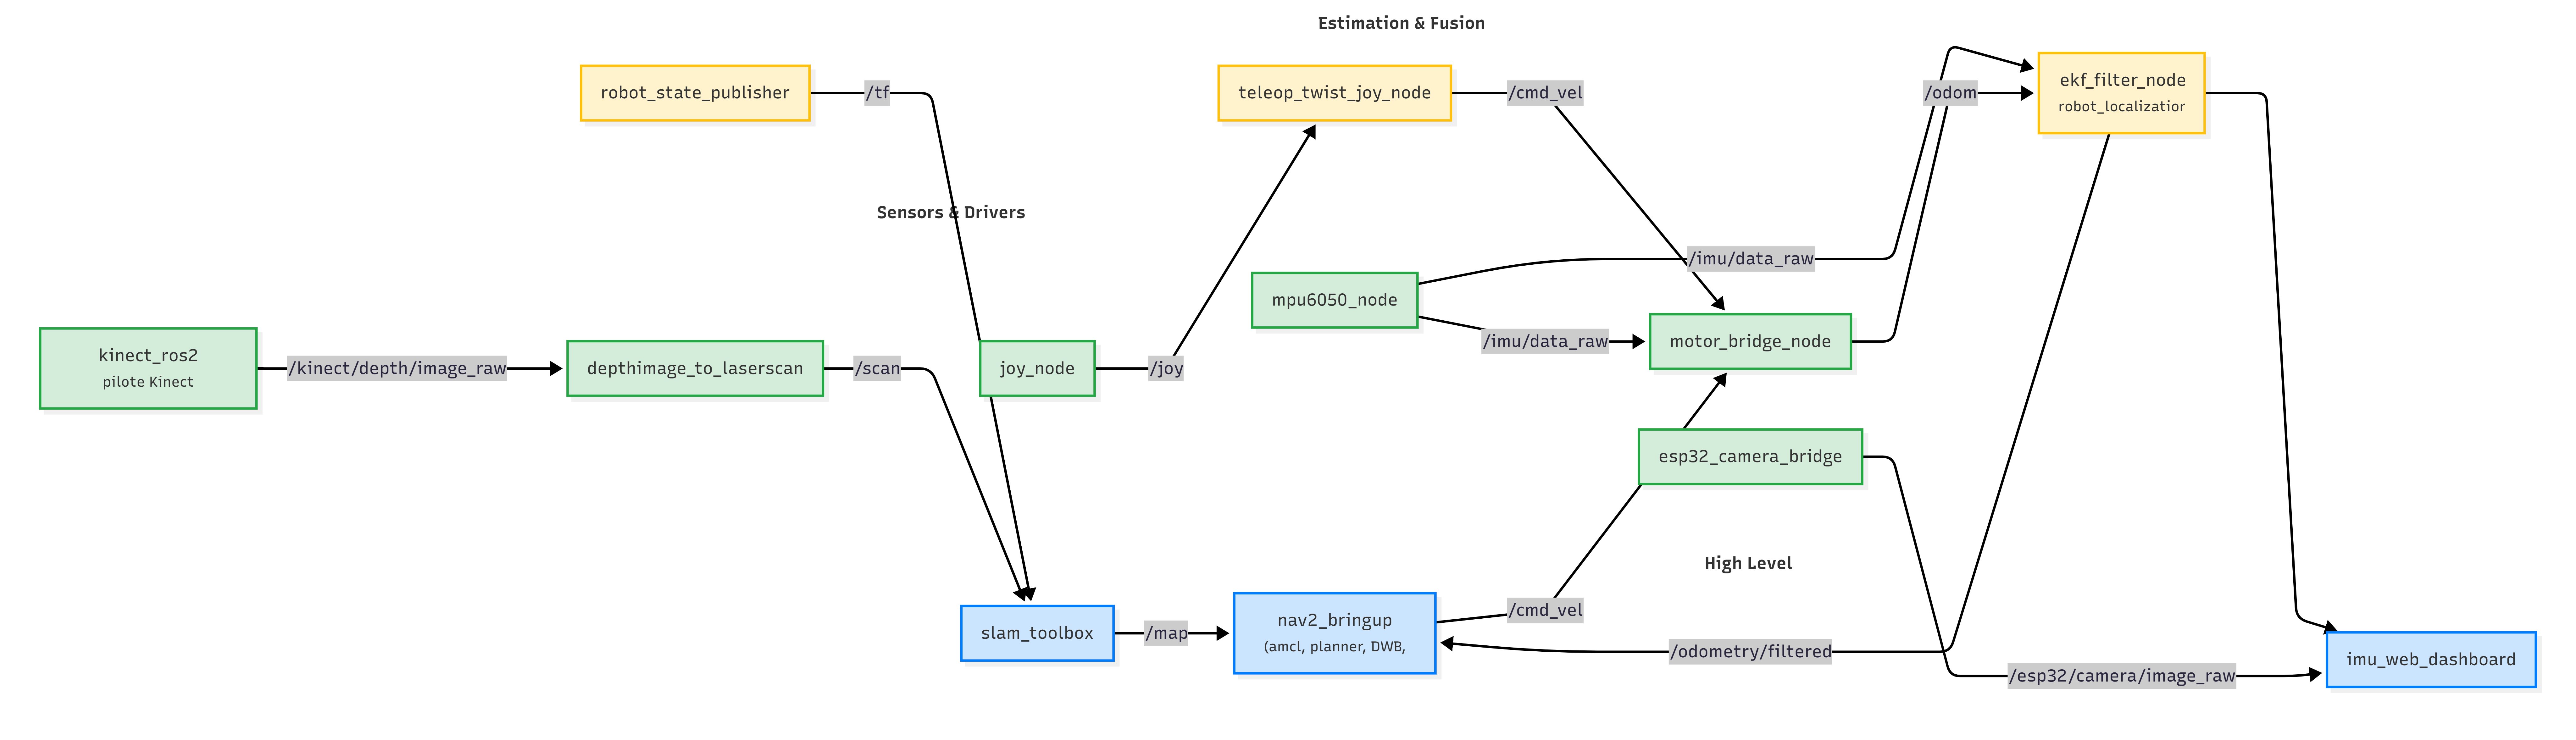
\includegraphics[width=0.78\linewidth]{images/Kinect_Stream.png}
	\caption{Graphe simplifié des noeuds et topics \ros{}\,2. Couleurs~: vert = pilotes capteurs/actionneurs,
		gris-bleu = estimation d'état, bleu = planification/cartographie haut-niveau.}
	\label{fig:topics_stream_spec}
\end{figure}

\section{Synthèse des topics principaux}
\label{sec:archi_topics_table}

Le tableau~\ref{tab:topics_summary} résume les topics \ros{}\,2 effectivement publiés ou
souscrits dans le code source. La liste exhaustive, avec types de message complets, est
fournie en annexe~\ref{app:topics}.

\begin{table}[H]
	\centering
	\caption{Topics \ros{}\,2 principaux --- architecture telle que construite.}
	\label{tab:topics_summary}
	\begin{tabularx}{\linewidth}{L{3.4cm} L{3.4cm} L{3.4cm} L{3.1cm}}
		\toprule
		\textbf{Topic} & \textbf{Type} & \textbf{Publié par} & \textbf{Souscrit par} \\
		\midrule
		\topic{/cmd\_vel} & geometry\_msgs/Twist & teleop\_twist\_joy, Nav2 & motor\_bridge\_node \\
		\topic{/odom} & nav\_msgs/Odometry & motor\_bridge\_node & ekf\_filter\_node \\
		\topic{/odometry/filtered} & nav\_msgs/Odometry & ekf\_filter\_node & Nav2, imu\_web\_dashboard \\
		\topic{/imu/data\_raw} & sensor\_msgs/Imu & mpu6050\_node & motor\_bridge\_node, ekf\_filter\_node, dashboard \\
		\topic{/scan} & sensor\_msgs/LaserScan & depthimage\_to\_laserscan (Kinect) & slam\_toolbox, Nav2 costmaps \\
		\topic{/map} & nav\_msgs/OccupancyGrid & slam\_toolbox & Nav2, \gls{rviz} \\
		\topic{/tf}, \topic{/tf\_static} & tf2\_msgs/TFMessage & robot\_state\_publisher, ekf, slam\_toolbox & Nav2, \gls{rviz} \\
		\topic{/joy} & sensor\_msgs/Joy & joy\_node & teleop\_twist\_joy\_node, dashboard \\
		\topic{/esp32/camera/image\_raw} & sensor\_msgs/Image & esp32\_camera\_bridge & (consommateur optionnel) \\
		\bottomrule
	\end{tabularx}
\end{table}
